\documentclass[onecolumn]{IEEEtran}

%% INCLUDING THE PREAMBLE
%%%%%%%%%%%%%%%%%%%%%%%%%%%%%%%%%%%%%%%%%%%%%%%%%%%%%%%%%%%%%%%%%%%%%%%%%%%
%                                                                         %
%                                 PREAMBLE                                %
%                                                                         %
%%%%%%%%%%%%%%%%%%%%%%%%%%%%%%%%%%%%%%%%%%%%%%%%%%%%%%%%%%%%%%%%%%%%%%%%%%%

%% PACKAGES
\usepackage[]{lineno}
%\linenumbers
\usepackage[usenames,dvipsnames]{xcolor}
\usepackage{microtype}
\usepackage[obeyDraft]{todonotes}
\usepackage{fancyvrb}
\VerbatimFootnotes
\usepackage{algorithmic}

%% GRAPHICS RELATED
\usepackage{graphicx}
\usepackage[outdir=./tmp/]{epstopdf}
\graphicspath{{../images/}{./}{./tmp/}}
\DeclareGraphicsExtensions{.eps, .pdf, .jpeg, .png,}

%% CPATION SETUP
\usepackage{float}
\usepackage{caption}
\usepackage{subcaption}
\captionsetup{belowskip=12pt,aboveskip=4pt}


%% BIBLIOGRAPHY
\bibliographystyle{ieeetr}

%% UNITS
\usepackage{siunitx}

%% EQUATIONS
\usepackage{amsmath}
%\numberwithin{equation}{section}

%% HYPERLINKS
\usepackage[debug]{hyperref}

%%%%%%%%%%%%%%%%%%%%%%%%%%%%%%%%%%%%%%%%%%%%%%%%%%%%%%%%%%%%%%%%%%%%%%%%%%%
%                                                                         %
%                             Listing Setup                               %
%                                                                         %
%%%%%%%%%%%%%%%%%%%%%%%%%%%%%%%%%%%%%%%%%%%%%%%%%%%%%%%%%%%%%%%%%%%%%%%%%%%
\usepackage{listings}
\lstset{ %
    language=C++,
    basicstyle=\footnotesize\ttfamily,
    numbers=left,
    numberstyle=\tiny\color{gray},
    stepnumber=2,
    numbersep=5pt,
    backgroundcolor=\color{white},
    showspaces=false,
    showstringspaces=false,
    showtabs=false,
    frame=single,
    rulecolor=\color{black},
    tabsize=2,
    breaklines=true,
    breakatwhitespace=false,
    title=\lstname,
    keywordstyle=\color{blue},
    commentstyle=\color{OliveGreen},
    stringstyle=\color{orange}
}
\DeclareCaptionFont{white}{\color{white}}
\DeclareCaptionFormat{listing}{\colorbox[cmyk]{0.43, 0.35, 0.35, 0.01}{\parbox{\dimexpr\textwidth-2\fboxsep\relax}{#1#2#3}}}
\captionsetup[lstlisting]{format=listing,labelfont=white,textfont=white,singlelinecheck=false,margin=0pt,font={bf,footnotesize}}
%\lstnewenvironment{code}[1][]%
%{ \noindent\minipage{\linewidth}
%	\lstset{#1}
%}
%{\endminipage}
%% USER COMMANDS
\usepackage{isotope}
\newcommand{\iso}{\isotope}
\newcommand{\figurewidth}{\textwidth}
\newcommand{\micron}{$\mu$m}



%% SUBVERSION INFORMATION
\usepackage{svn-multi}
\svnidlong
{$LastChangedBy$}
{$LastChangedRevision$}
{$LastChangedDate$}
{$HeadURL$}

%%%%%%%%%%%%%%%%%%%%%%%%%%%%%%%%%%%%%%%%%%%%%%%%%%%%%%%%%%%%%%%%%%%%%%%%%%%
%                                                                         %
%                                Start of Document                        %
%                                                                         %
%%%%%%%%%%%%%%%%%%%%%%%%%%%%%%%%%%%%%%%%%%%%%%%%%%%%%%%%%%%%%%%%%%%%%%%%%%%
\begin{document}
\title{Comparison of Lithiated Glass, LiF:ZnS(Ag), Boron Loaded Plastic, PEN, and PS Detectors}
\author{Matthew J. Urffer}
\date{\today}
\maketitle

% Tables of Contents, Figures, Tables
\tableofcontents
\listoffigures
\listoftables
%%%%%%%%%%%%%%%%%%%%%%%%%%%%%%%%%%%%%%%%%%%%%%%%%%%%%%%%%%%%%%%%%%%%%%%%%%%
%                                                                         %
%                              Start of Content                           %
%                                                                         %
%%%%%%%%%%%%%%%%%%%%%%%%%%%%%%%%%%%%%%%%%%%%%%%%%%%%%%%%%%%%%%%%%%%%%%%%%%%
\section{Introduction}

The potential application  of a material for use in a Radiation Portal Monitor (RPM) can be evaluated by measurements of the detector's sensitivity to gammas and the detector's response to neutrons.
A detector material might be a possible replacement if the there exists a neutron response that can be differentiated from photons for given sensitivity of gammas, namely \num{1E-6}.
A simple way to discriminate between gammas and neutrons is to use a pulse height discriminator, above which the detector detector will only record one photon out a million as a neutron.
Under this framework it is then possible to develop a mathematical lower level discriminator (MLLD) of the pulse height spectrum to function as this pulse height discriminator, and to then formulate the sensitivity requirement as the gamma intrinsic efficiency as a function of MLLD.
Six detectors (three boron loaded plastic scintillators, one LiF:ZnS(Ag) doped screen, GS20, a post processed composite PEN film\footnote{Sample was 22-March-2013, 25\% LiF, 70\% PEN, 5\% PPO-POPOP post processed}, and a polystyrene\footnote{Sample was cast 24 Jan 2012 at \SI{50}{\um} with 10\% LiF, 5\% PPO-POPOP, and 85\% PS}) were then evaluated for their ability to perform in a RPM. 
The thickness of these detectors and mass of the absorber are shown in \autoref{tab:PhysicalProperties}.
\begin{table}[h]
\centering
\caption[Detector Physical Characteristics]{Physical characteristics of the detector.}
\label{tab:PhysicalProperties}
  \begin{tabular}{m{4cm}| m{2cm} m{2cm} m{2cm}}
  \toprule
    & Absorber & Thickness &  Mass Absorber (mg) \\
    \midrule
    EJ 254 2.5\% & \iso[10]{B} & 1/4" & 59.5 \\
    EJ 254 1\% & \iso[10]{B} & 1/4" & 23.8 \\
    EJ 254 5\% & \iso[10]{B} & 3/4 & 356.1 \\
    EJ 425 HD2-PE & \iso[6]{Li} & \SI{0.1}{\mm} & 17.5 \\
    GS20 & \iso[6]{LI} & \SI{2}{\mm} & 155 \\
    Post processed Composite PEN Film (22 Mar)& \iso[6]{Li} & $\approx$ \SI{212}{\um} & 42.42 \\
    PS Film & \iso[6]{Li} & \SI{50}{\um} & 2.71 \\
    \bottomrule
  \end{tabular}
\end{table}

\subsection{Previous Work}

Work by Guerard (published slides) has the performance of GS20 and a LiF:ZnS film (\autoref{fig:GuerardLightYield}).
It should be noted that Guerard's measurement is not the same as ours - the neutron source is unknown, as well is the supplier of the LiF:ZnS film (and thickness). 
In addition, the thickness of GS20 reported by Guerard is \SI{0.5}{\mm} while the GS20 in the detection lab is \SI{2}{\mm}.
\begin{figure}
  \centering
  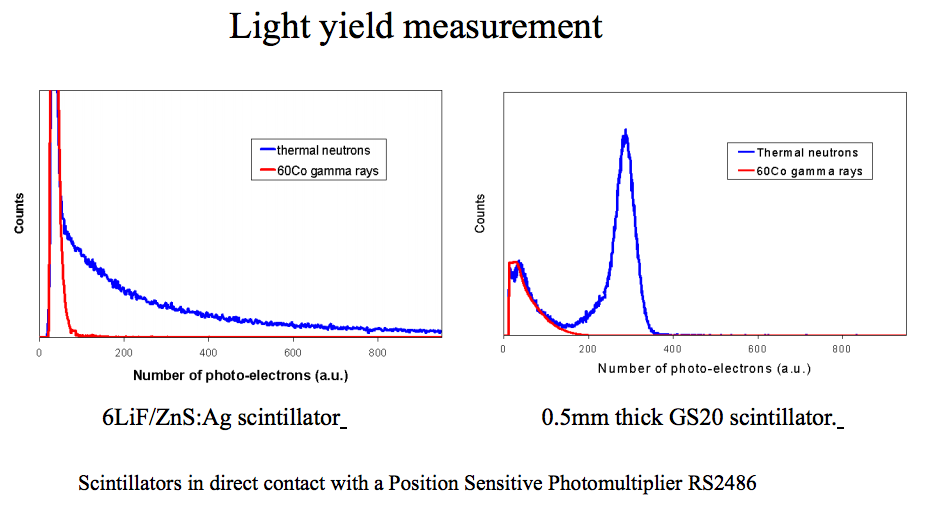
\includegraphics[width=\textwidth]{Guerard_LightYieldMeasurement}
  \caption[Measured Light Yield (Guerard)]{Light yield as measured by Guerard. The GS20 measurement has a lower gamma performance than as measured (in addition to lacking a Compton edge), and the LiF:ZnS \iso[60]{Co} spectra does not have the same shape as we measured}
	\label{fig:GuerardLightYield}
\end{figure}
\autoref{fig:GuerardIntEff} shows the neutron detection efficiency and sensitivity to \iso[60]{Co} photons.
For a sensitivity of \num{1E-6} the LiF:ZnS film is reported to have a neutron detection efficiency of 60\%, while the \SI{1}{\mm} GS20 has a reported neutron detection efficiency of 55\%.
Detection efficiency in this case is equatable to the probability of absorption.
\begin{figure}
  \centering
  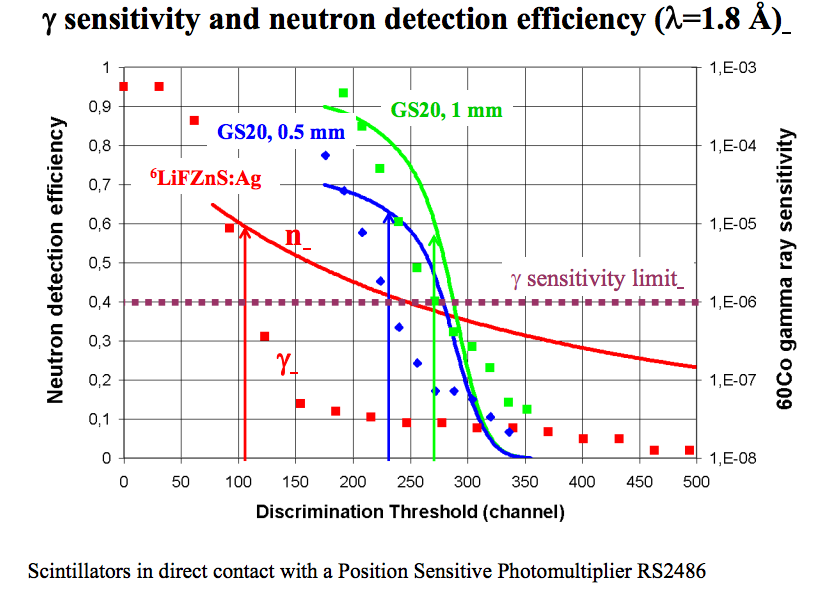
\includegraphics[width=\textwidth]{Guerard_IntEff_NCr}
  \caption[Intrinsic Efficiency (Geurard)]{Intrinsic Efficiency of LiF:ZnS and GS20 from Guerard.  The gamma intrinsic efficiency is shown in the solid squares (right axis), while the lines show the neutron efficiency (left axis). The values reported here are much higher than the values reported in this report.}
	\label{fig:GuerardIntEff}
\end{figure}

\section{Methods}
The neutron performance was determined by the \iso[252]{Cf} irridiator previously described, and the gamma source was the \iso[60]{Co} irridiator.
Due to the wide range of light output of these films it was necessary to use a two voltages (\SI{1000}{\volt} and \SI{1180}{\volt}) in order to capture the entire spectra on an ADC with a zero to \SI{10}{\volt} range with repeatable resolution.
However, a measurement of the GS20 peak in the lead well was always recorded which then allowed the spectra to be tied together based on this feature, as shown in \autoref{eqn:SettingScale}.
\begin{align}
  \label{eqn:SettingScale}
  \text{Channel Feature at Setting A} = \frac{\text{Channel GS20 Peak at Setting A}}{\text{Channel GS20 Peak at Setting B}} \;\; \left( \text{Channel Feature at Setting B}\right)
\end{align}
The count rates are not scaled for gain and voltage settings as they should remain constant as long as counts are not pushed below the lower level discriminator or cause roll-off.
\subsection{Neutron Performance above Gamma Discriminator}
An accurate measure of the neutron performance above the pulse height discriminator is essential for the comparison between detector materials.
In \autoref{fig:GammaMLLDIntEff} it is shown that the location of the MLLD is a pretty stable measurement for PS films of a different thickness.
\begin{figure}
  \centering
  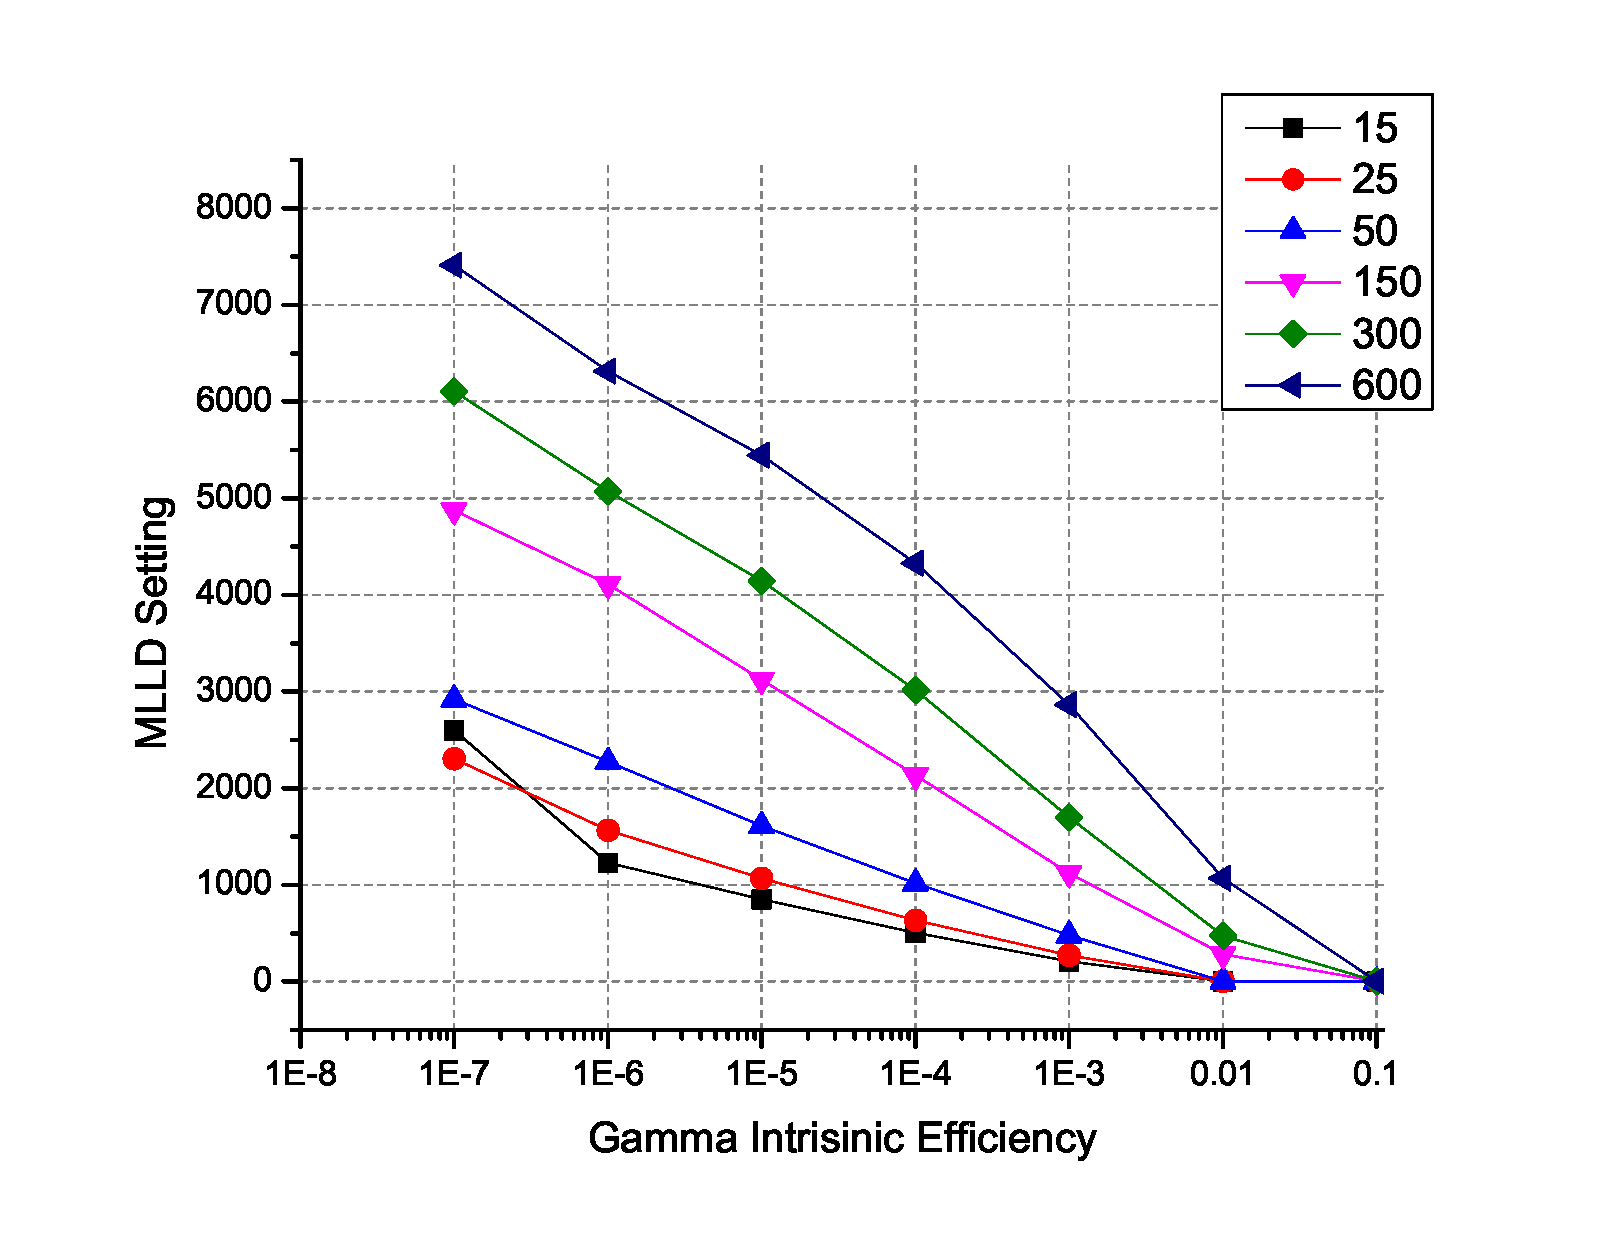
\includegraphics[width=\textwidth]{PS_IntEffMLLD_LiF}
  \caption[Stability of Lower Level Discriminator]{The mathematical lower level discriminator (MLLD) as a function of intrinsic effigies for 10\% PS films of various thickness. The linear nature suggest that the determination of the MLLD is repeatable.}
  \label{fig:GammaMLLDIntEff}
\end{figure}
However, in previous work which focused on using the fraction of neutron counts above the MLLD it was observed that the fraction (as it is normalized by the entire count rate) is very susceptible to sample to sample variations in the low energy channels.
Therefore, after extensive studies using the polystyrene matrix a more stable measure was found by simply integrating the counts in the neutron spectra above the MLLD and then normalizing by the mass of neutron absorber in the samples (\autoref{eqn:CountRateAbovePerMass}).
While this method does not have the errors associated with summing over the low channels, it does require an accurate measure of the mass of \iso[6]{Li} in the sample.
Alternative methods would also probably be stable, but they are not discussed here.
\begin{align}
\label{eqn:CountRateAbovePerMass}
\eta = \frac{\int_{\text{MLLD}}^\infty p(x)dx}{\text{Neutron Absorber Mass}}
\end{align}

\section{Results}
The following figures, \autoref{fig:Co60Spectra} and \autoref{fig:PbWellSpectra}, show the measured spectra of the detectors for neutrons and gammas.
It is clear that the EJ-254 (boron loaded plastic) detectors will have poor performance because of their large gamma response.
The EJ-426 (LiF:ZnS(Ag)) has the lowest response, and it is not clear if the tail of the spectra is due to actual counts or background.
In the neutron spectra it was decided to only plot the performance of the best EJ-254 (though \autoref{fig:EJ254Perf} display the performance of all EJ-254 films).
It is observed that the LiF:ZnS(Ag) is much brighter than the other films, and it is noted that the post processed composite PEN has a higher light output than the commercial EJ-254 (based on the peak location).
\begin{figure}
  \centering
  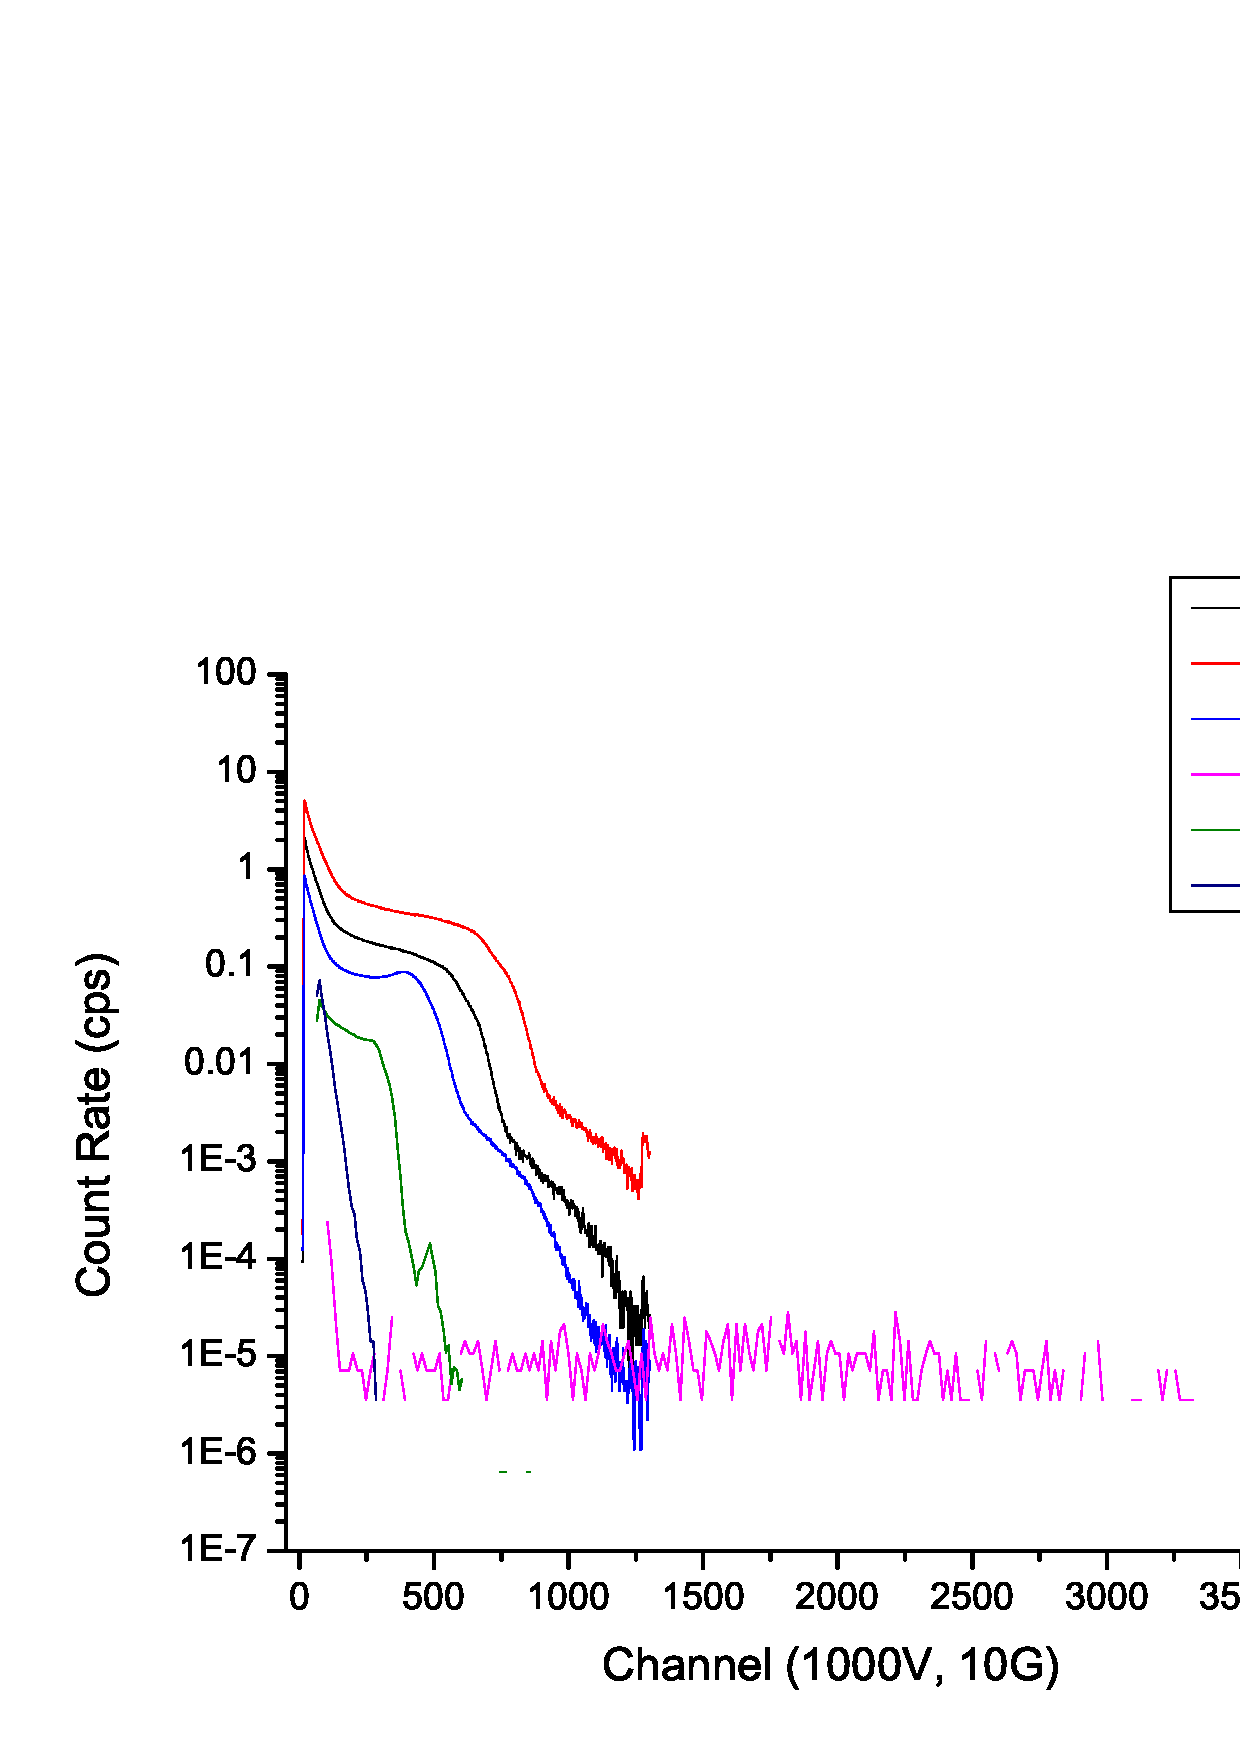
\includegraphics[width=\textwidth]{SampleComparions_Co60Spectra}
  \caption[Gamma Response of Measured Detectors]{Gamma Response from \iso[60]{Co} source of measured detectors.}
  \label{fig:Co60Spectra}
\end{figure}
\begin{figure}
  \centering
  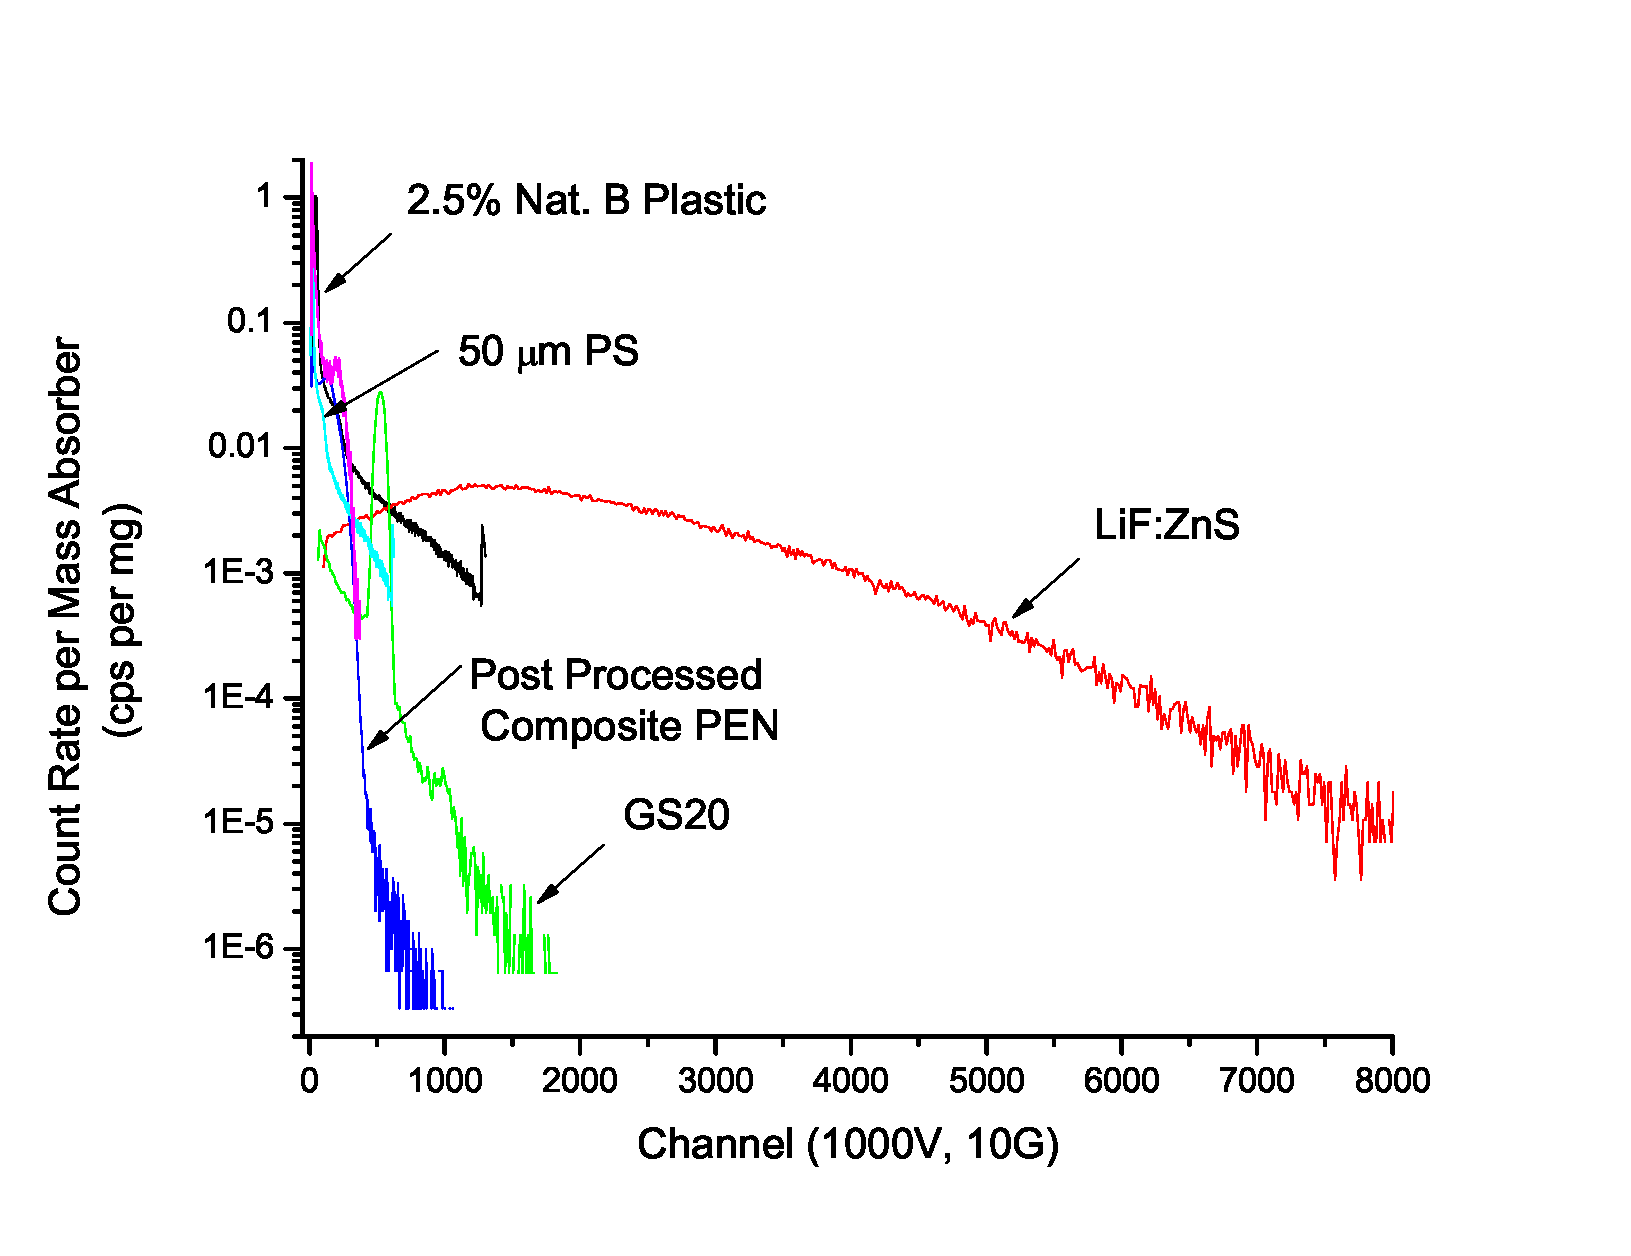
\includegraphics[width=\textwidth]{SampleComparison_PbCRperMg}
  \caption[Neutron Response of Measured Detectors]{Neutron Response (lead well) of the measured detectors. The count rate has been normalized by the mass of neutron absorber in the detector.}
  \label{fig:PbWellSpectra}
\end{figure}
The average channel number of the neutron and gamma spectra of each detector was calculated and are presented in \autoref{tab:AvgChNG}.
The average was computed for the neutrons in the thermal well to avoid the low energy channels from shifting the spectra away from any peak location.
It should be noted that for EJ-254 the low channel number average is correct; this feature was identified as the neutron peak.
Eljen publishes the light yield for the 1\% boron as 9,200 photons per MeVee, 8,600 photons per MeVee for the 2.5\% boron, and 7,500 photons per MeVee for the 5\% boron, and \autoref{tab:AvgChNG} shows agreement to these values.
C.W.E van Eijk has published the light yield of LiF:ZnS as 75,000 photons per MeVee, which is close to our measured value of 72,000 photons per MeVee.
\begin{table}
  \centering
  \caption[Average Channel Number of Gamma and Neutron Spectra]{Average channel number of gamma and the thermal neutron spectra.  The channel averages are scaled to 1,000V, 10G. The light yields are scaled to GS20 having 3,800 photons per MeV, and 6,250 photons per Neutron.}
  \label{tab:AvgChNG}
  \begin{tabular}{c| c c |c c}
    \toprule
        &\multicolumn{2}{|c|}{Gamma}&\multicolumn{2}{|c}{Neutron}\\
        & Average Channel& Photons per MeVee & Average Neutron Channel & Photons per Neutron\\
    \midrule
    EJ 254 2.5\%, 1/4"&	183.41	&	8,100	&	54.06	&	640	\\
    EJ 254 1\%, 1/4"&	216.25	&	9,500	&	65.04	&	780	\\
    EJ 254 5\%, 3/4"&	176.49	&	7,800	&	39.56	&	479	\\
    EJ 426 HD2&	1636.53	&	72,000	&	2018.46	& 	24,000	\\
    GS20 &	172.76	&	3800.00	&	524.10	&	6,250	\\
    Post processed Composite PEN & 41.11 & 1,800 & 142.01 & 1,700\\
    PS Film & 32.18 & 1,400 & 169.34 & 2,000 \\
    \bottomrule
  \end{tabular}
\end{table}
The count rates of the detectors are presented in \autoref{tab:CountRate} for both the thermal component as well as only in the lead well spectra.
\begin{table}
\centering
  \caption[Detector Count Rate]{Count rate of the detectors in the thermal spectra as well as the lead well spectra.  The final two columns are normalize by the mass of the absorber in the material. Significant self-shielding may exists in the the 5\% boron, 3/4" EJ-254.}
  \label{tab:CountRate}
  \begin{tabular}{p{2cm} | c c| c c}
  \toprule
    &\multicolumn{2}{|c|}{Count Rate (cps)}&\multicolumn{2}{|c}{Count Rate per Mass Absorber (cps per mg)} \\
    & Thermal Neutrons &Lead Well & Thermal Neutrons & Lead Well\\
  \midrule
  EJ 254 2.5\%, 1/4"&	1104	&	1869	&	18.5	&	31.4	\\
  EJ 254 1\%, 1/4"&	447	&	1130	&	18.8	&	47.5	\\
  EJ 254 5\%, 3/4"&	1417	&	3415	&	3.98	&	9.59	\\
  EJ 42 6 HD2 \SI{0.1}{\mm}&	224	&	234	&	12.8	&	13.4	\\
  GS20 \SI{2}{\mm}&	328	&	412	&	2.12	&	2.66	\\
  Post processed Composite PEN $\approx$ \SI{212}{\um}&	322	& 227	&	5.35 &	7.60	\\
  PS, \SI{50}{\um}, 10\% LiF & 90.6 & 20.7 & 7.63& 33.4 \\
  \bottomrule
  \end{tabular}
\end{table}
\autoref{tab:DiscrimPreformance} shows the discrimination performance of the tested detectors, while \autoref{fig:DiscrimPerformance} plots the intrinsic efficiency (sensitivity) along with the neutron count rate, normalized by the absorber mass.
\begin{table}
  \centering
  \caption[Discrimination Performance]{Discriminator setting and count rate above the gamma intrinsic efficiency of \num{1E-6} for various detectors.}
  \label{tab:DiscrimPreformance}
  \begin{tabular}{m{5cm} | m{2cm} m{6cm}}
    \toprule
    &	MLLD Location	&	Count Rate above the intrinsic discriminator setting of \num{1E-6} per Absorber Mass (cps per mg)	\\
    \midrule
    EJ 254, 2.5\% B, 1/4"	&	1280	&	0.20	\\
    EJ 254, 1\% B, 1/4"	&	1300	&	0.05	\\
    EJ 254, 5\% B, 3/4"	&	1290		&	0.03	\\
    EJ 426 HD2, \SI{0.1}{\mm}&	3308		&	1.97	\\
    GS20, \SI{2}{\mm}	&	557		&	0.56	\\
    Post processed Composite PEN,\SI{212}{\um}, 25\% LiF	&	284	&	0.73	\\
    PS, \SI{50}{\um}, 10\% LiF & 223 & 2.15\\
    \bottomrule
\end{tabular}
\end{table}
\begin{figure}
  \centering
  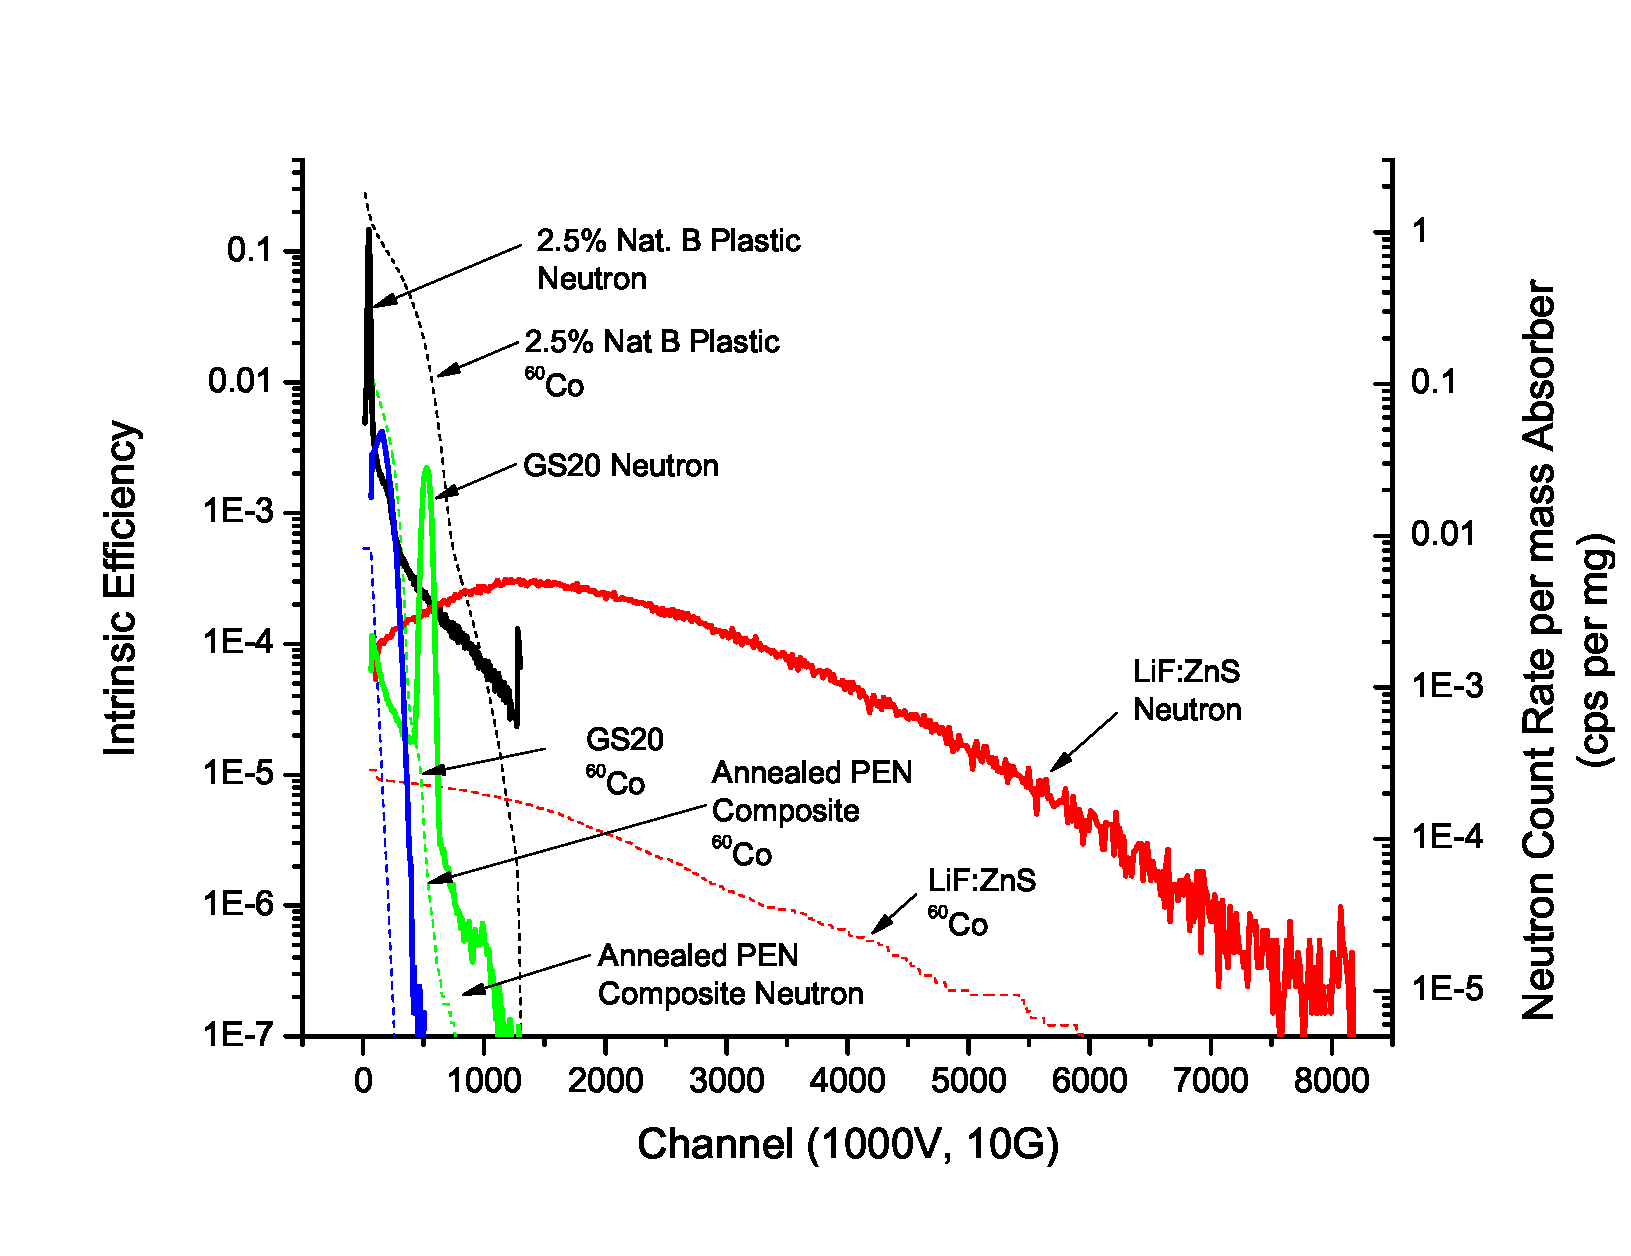
\includegraphics[width=\textwidth]{SampleComparison_IntEff_CR}
  \caption[Gamma Sensitivity and Neutron Response of Measured Detectors]{Gamma sensitivity (left axis, dashed lines) and neutron performance (right axis, solid lines) of measured detectors.  The neutron count rate above the gamma pulse height discriminator may be found by noting where the intrinsic efficiency crosses \num{1E-6} and then integrating the neutron spectra above it. The neutron spectra are from the lead well, and are normalized by the mass of absorber.}
  \label{fig:DiscrimPerformance}
\end{figure}
\autoref{fig:UTDetectorPreformance} demonstrates the performance of two detectors fabricated at UT (the PEN by Rohit Uppal and the PS by Andrew Mabe).
\begin{figure}
  \centering
  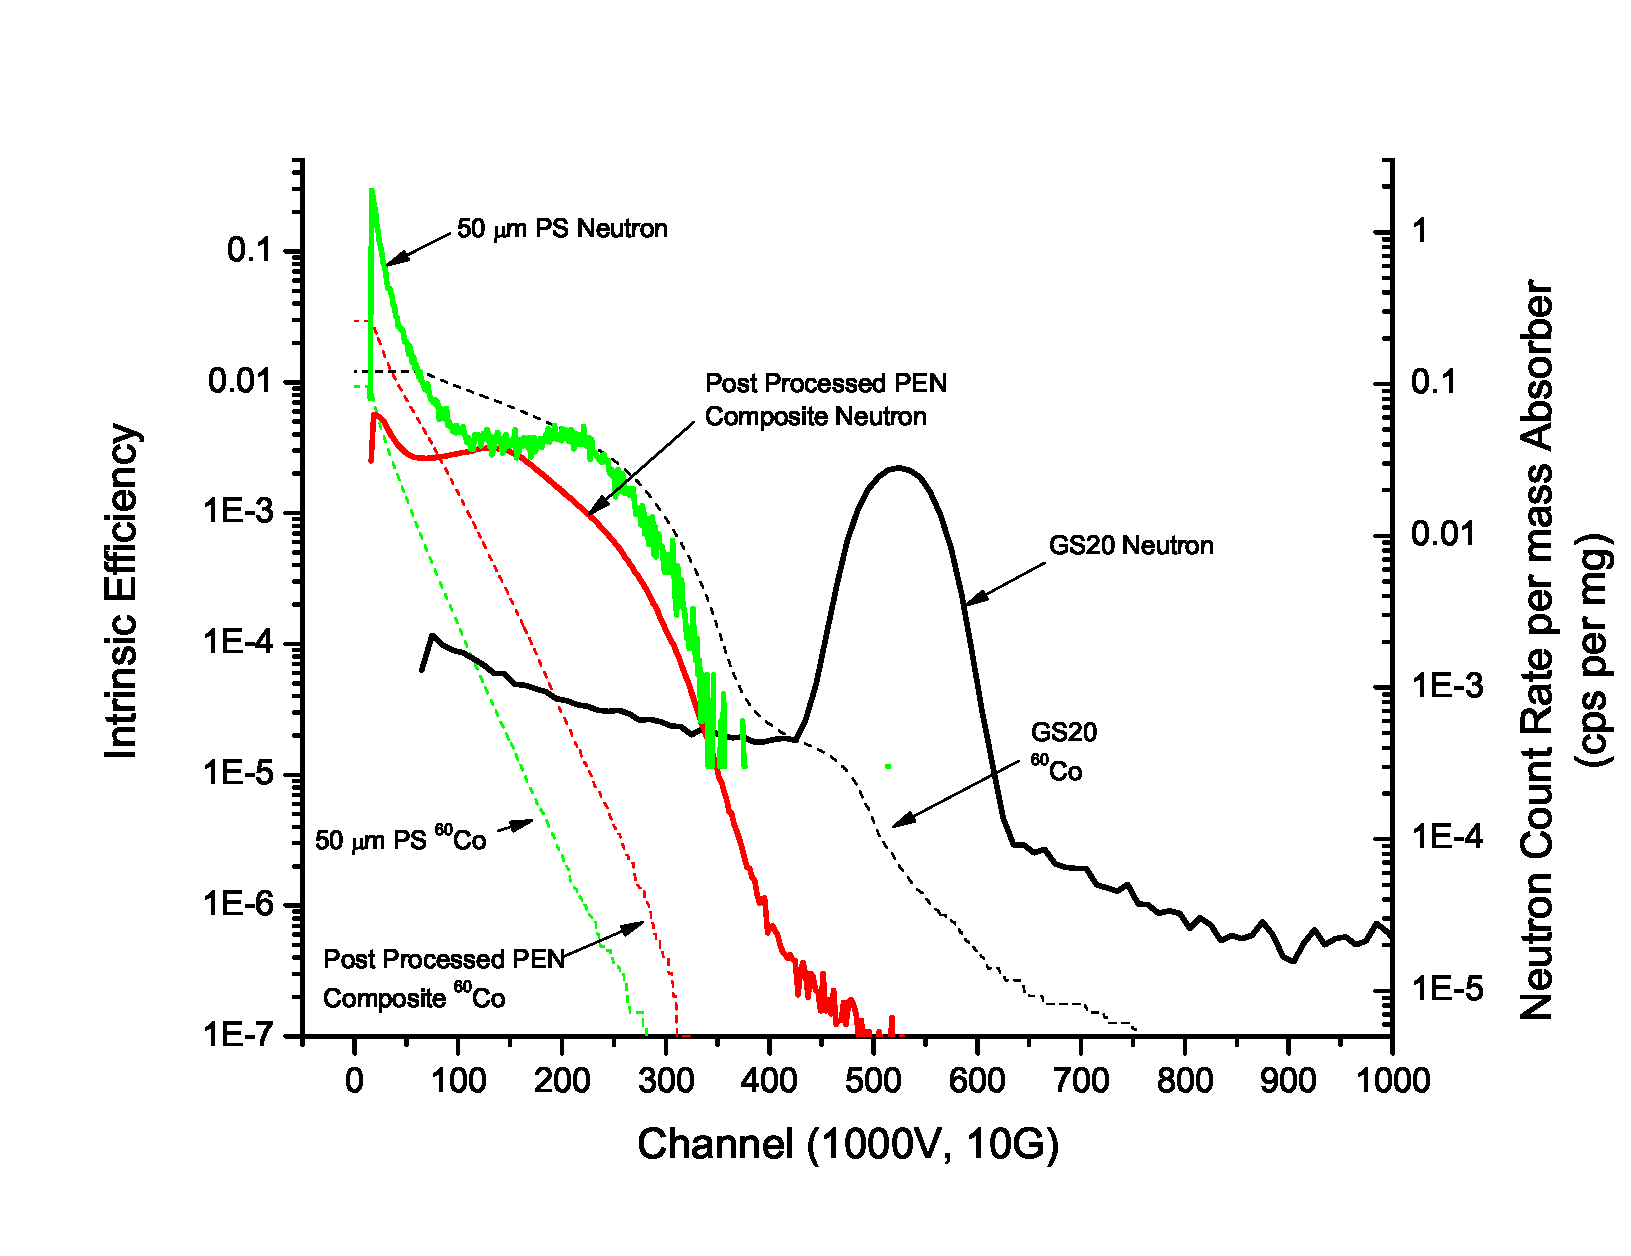
\includegraphics[width=\textwidth]{SC_UTDetectors_IntEff_CR}
  \caption[UT Fabricated Detector Performance]{Performance of a polystyrene and PEN film fabricated at UT compared to GS20.}
  \label{fig:UTDetectorPreformance}
\end{figure}

\subsection{Individual Detector Performance}
The performance of the individual detectors are shown in the separate figures to clearly illustrate important features.
\begin{figure}
  \centering
  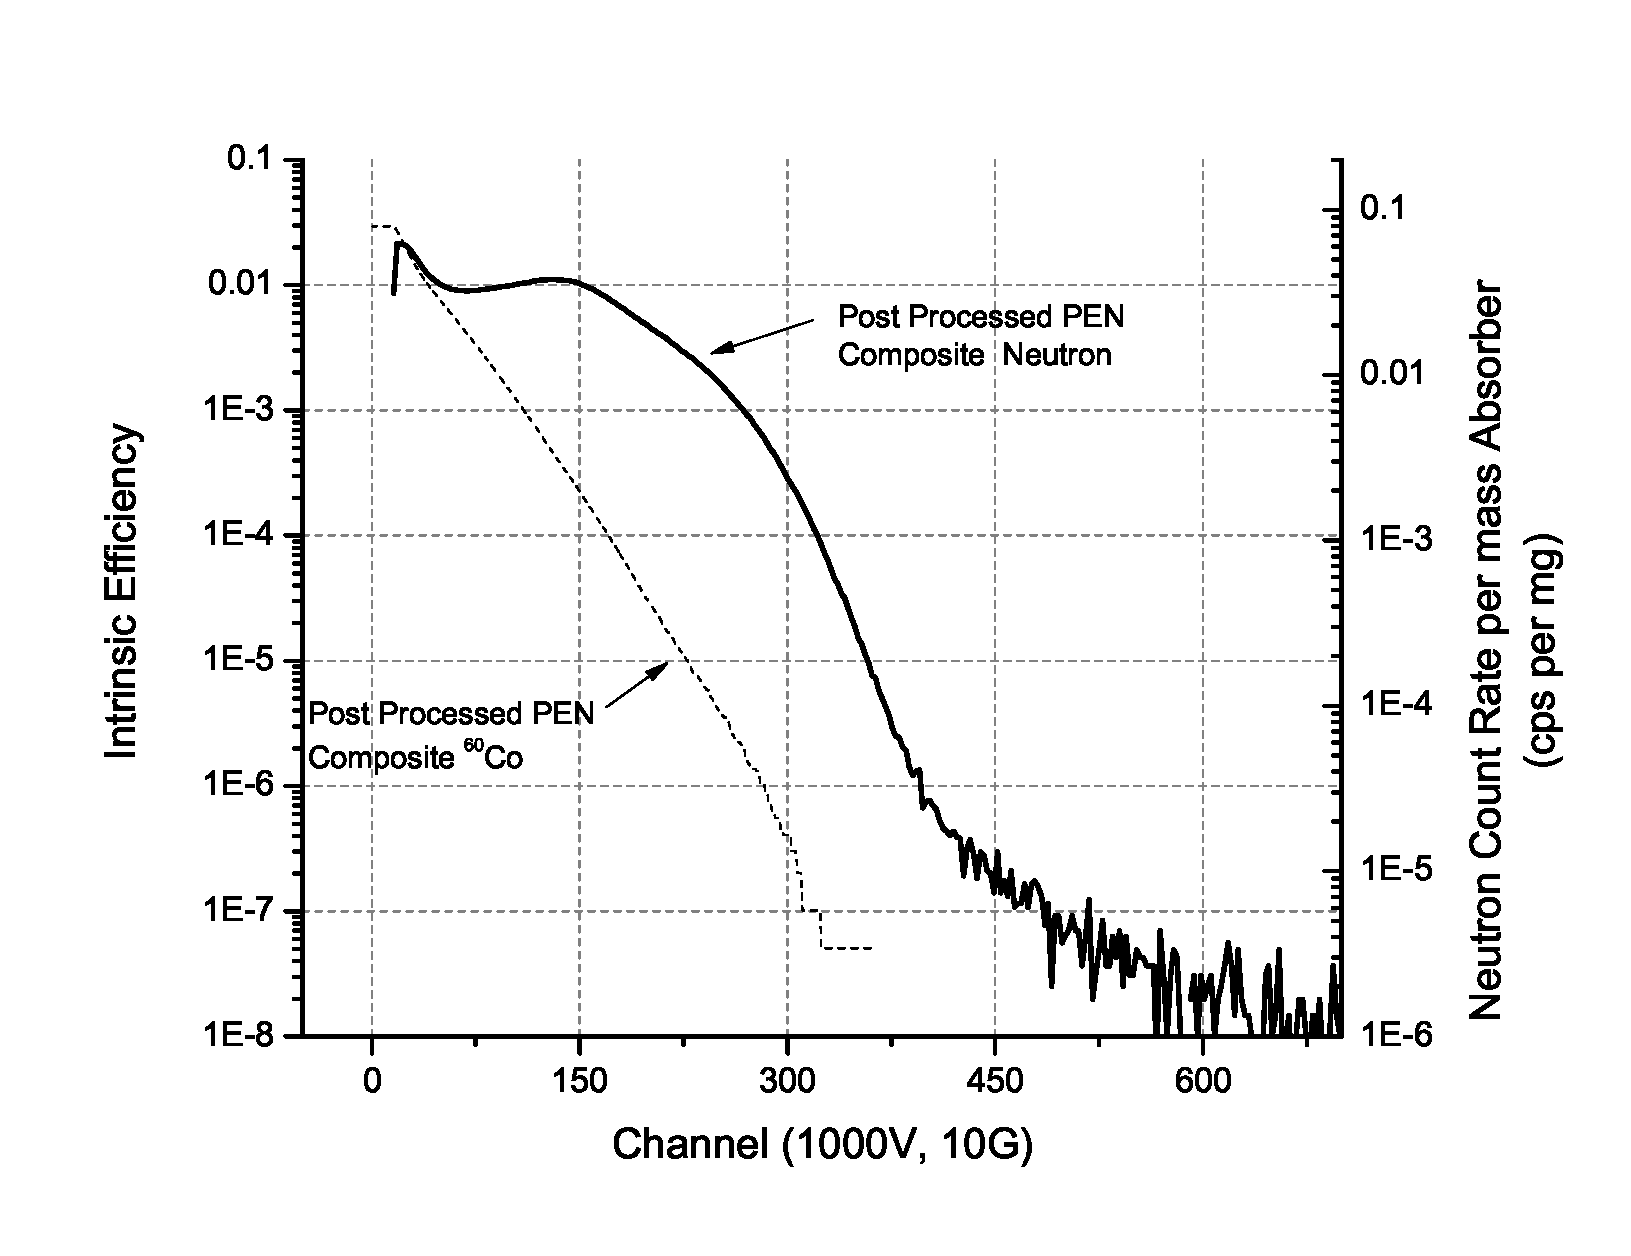
\includegraphics[width=\textwidth]{SC_ACPEN_IntEff_CR}
  \caption[Post processed Composite PEN Performance]{Performance of an Post processed Composite PEN Film (22 March Sample).}
  \label{fig:ACPENPreformance}
\end{figure}
\begin{figure}
  \centering
  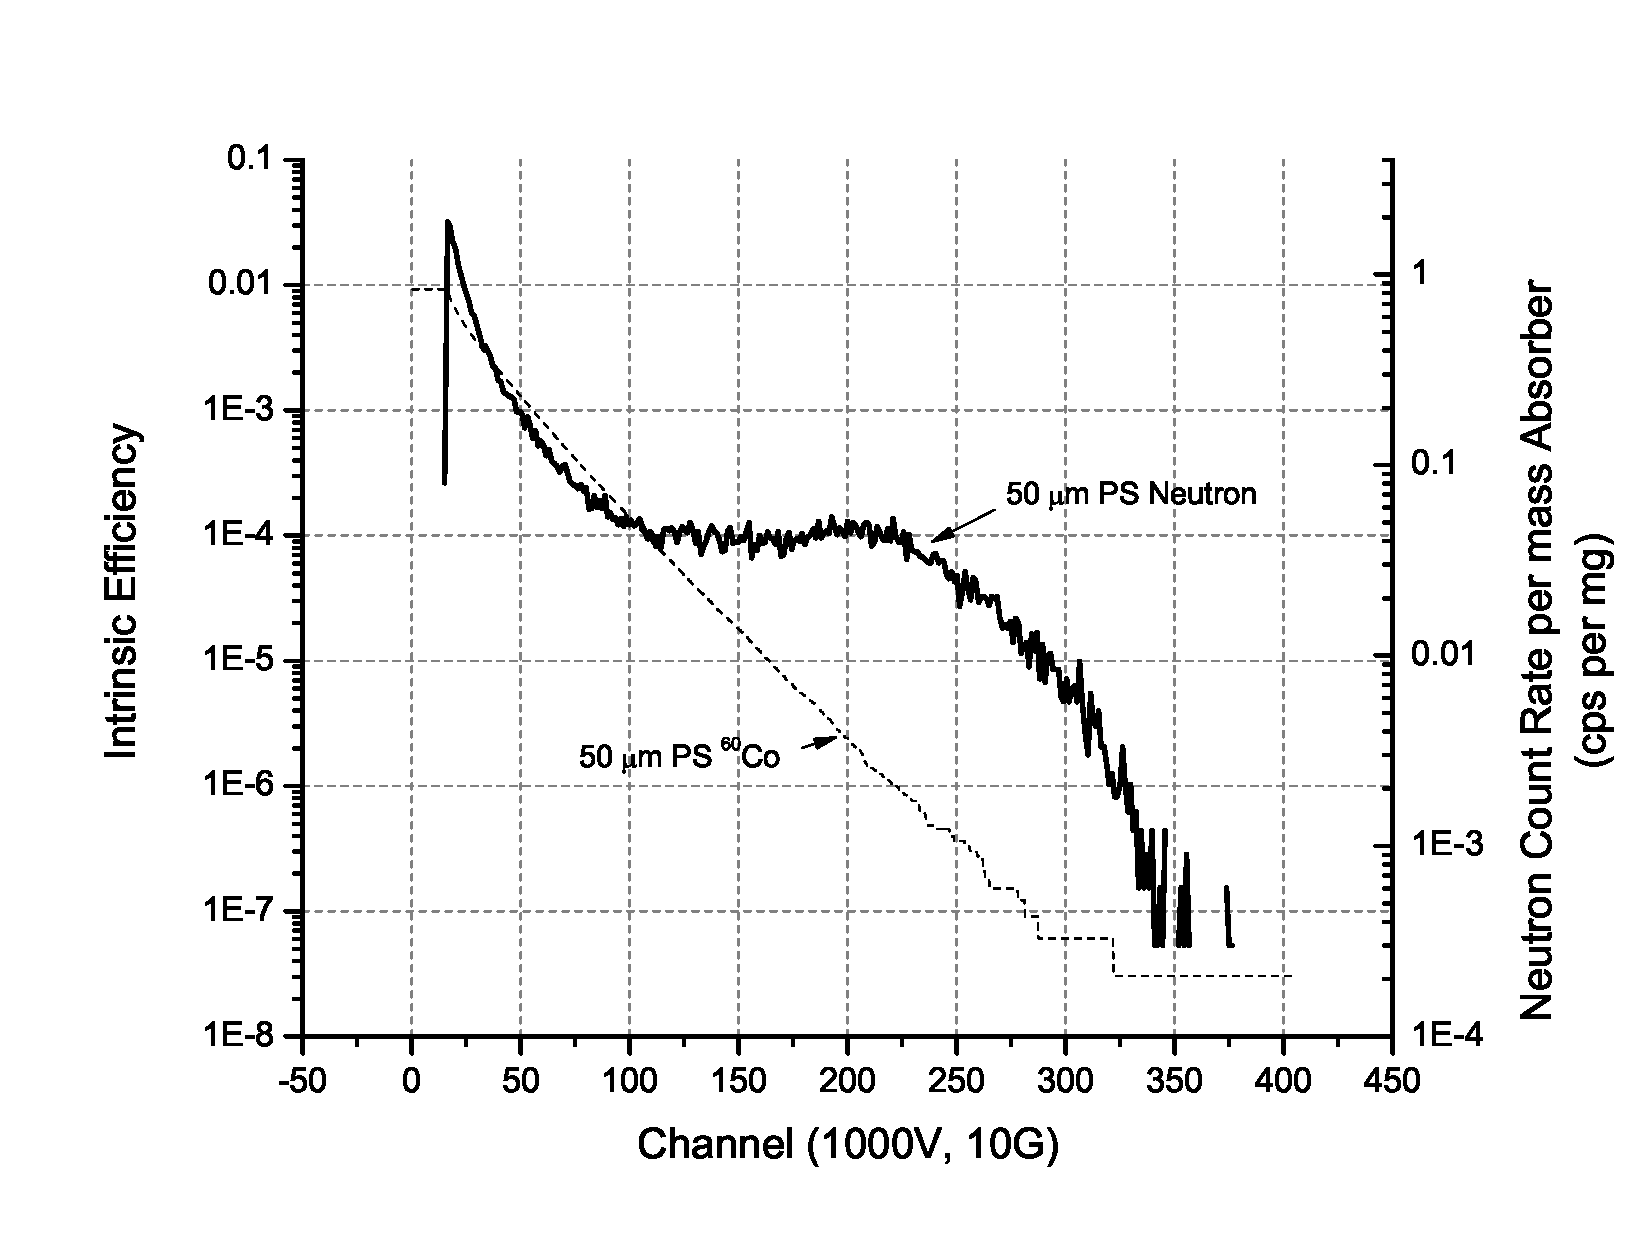
\includegraphics[width=\textwidth]{SC_PS_IntEff_CR}
  \caption[Cast Polystyrene Performance]{Performance of an \SI{50}{\um}, 10\% \iso[6]{LiF} PS Film (24 Jan 2012 Sample).}
  \label{fig:PSPreformance}
\end{figure}
\begin{figure}
  \centering
  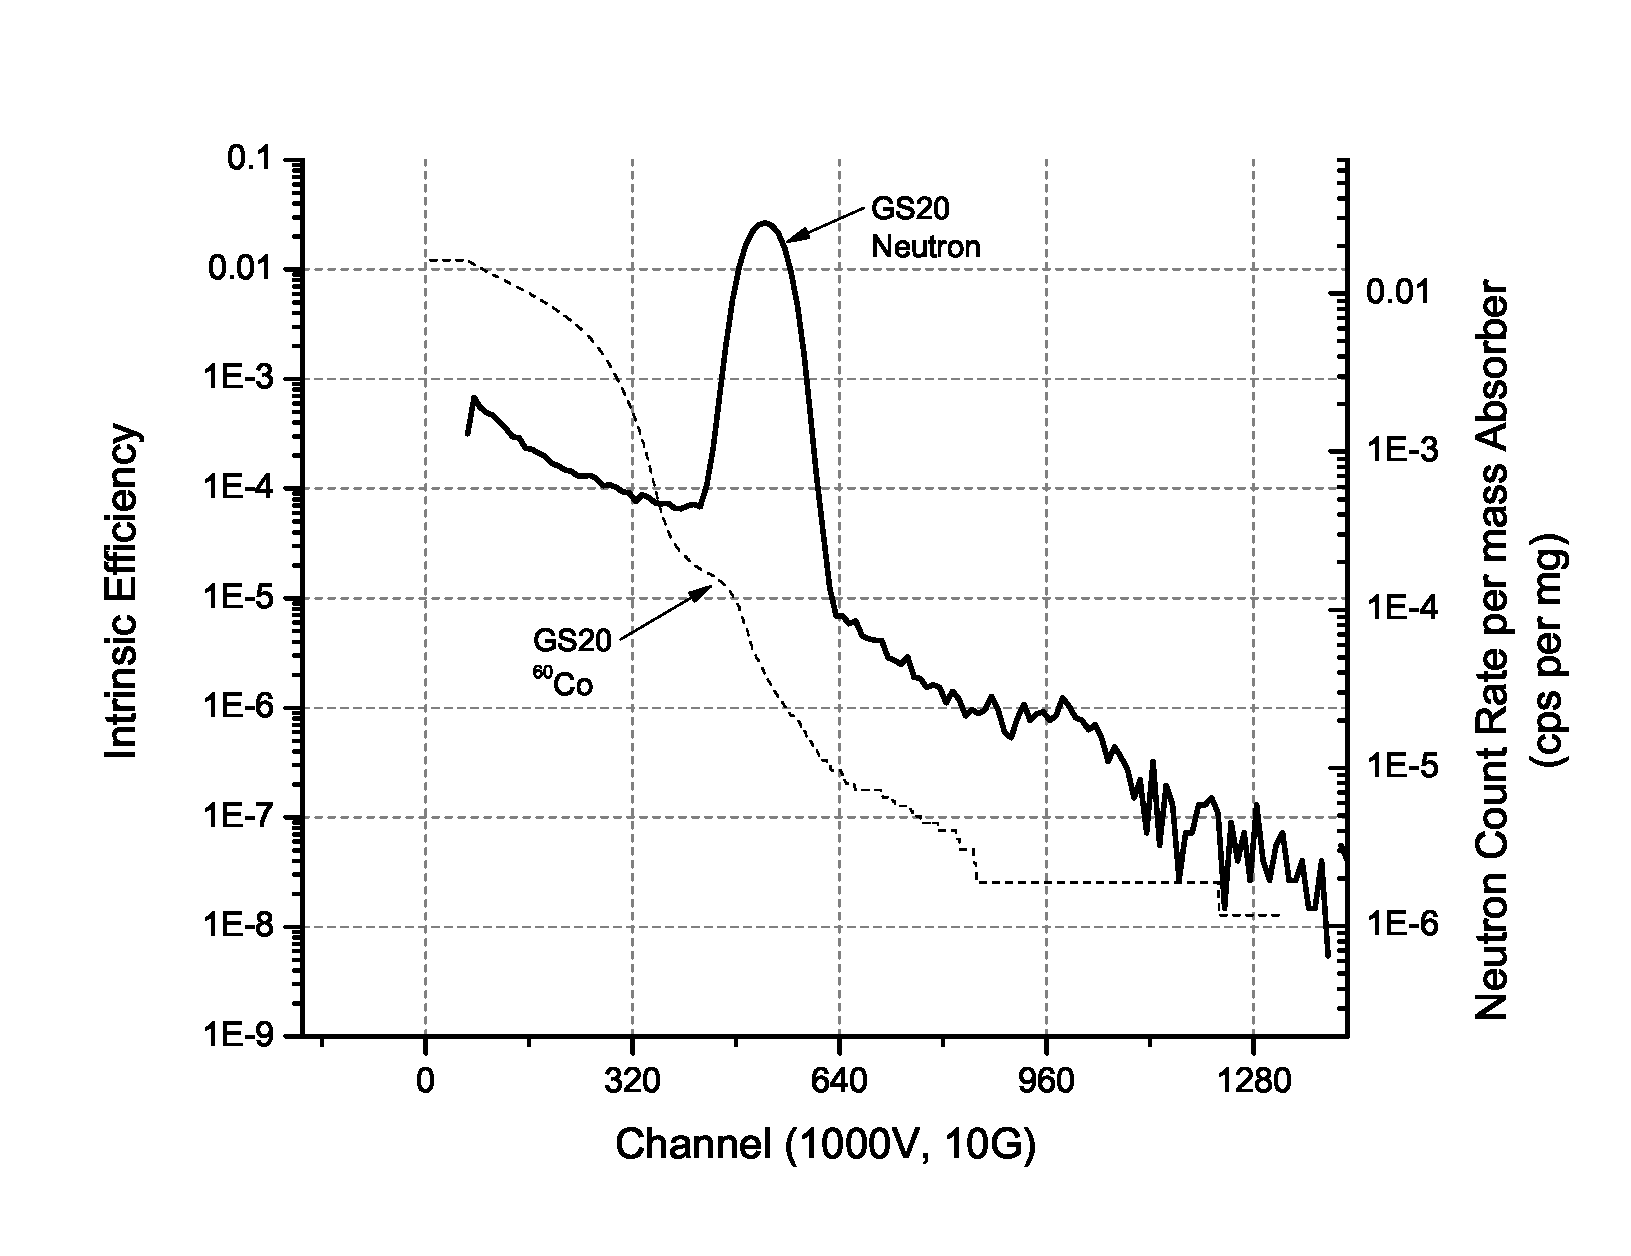
\includegraphics[width=\textwidth]{SC_GS20_IntEff_CR}
  \caption[GS20 Performance]{Performance of \SI{2}{\mm} GS20.  It should be noted that there is significant self shielding in GS20, and that due to the gamma sensitivity catching the tail of the neutron peak the count rate above the gamma pulse height discriminator has the most variation of the samples measured.}
  \label{fig:GS20Preformance}
\end{figure}
\begin{figure}
  \centering
  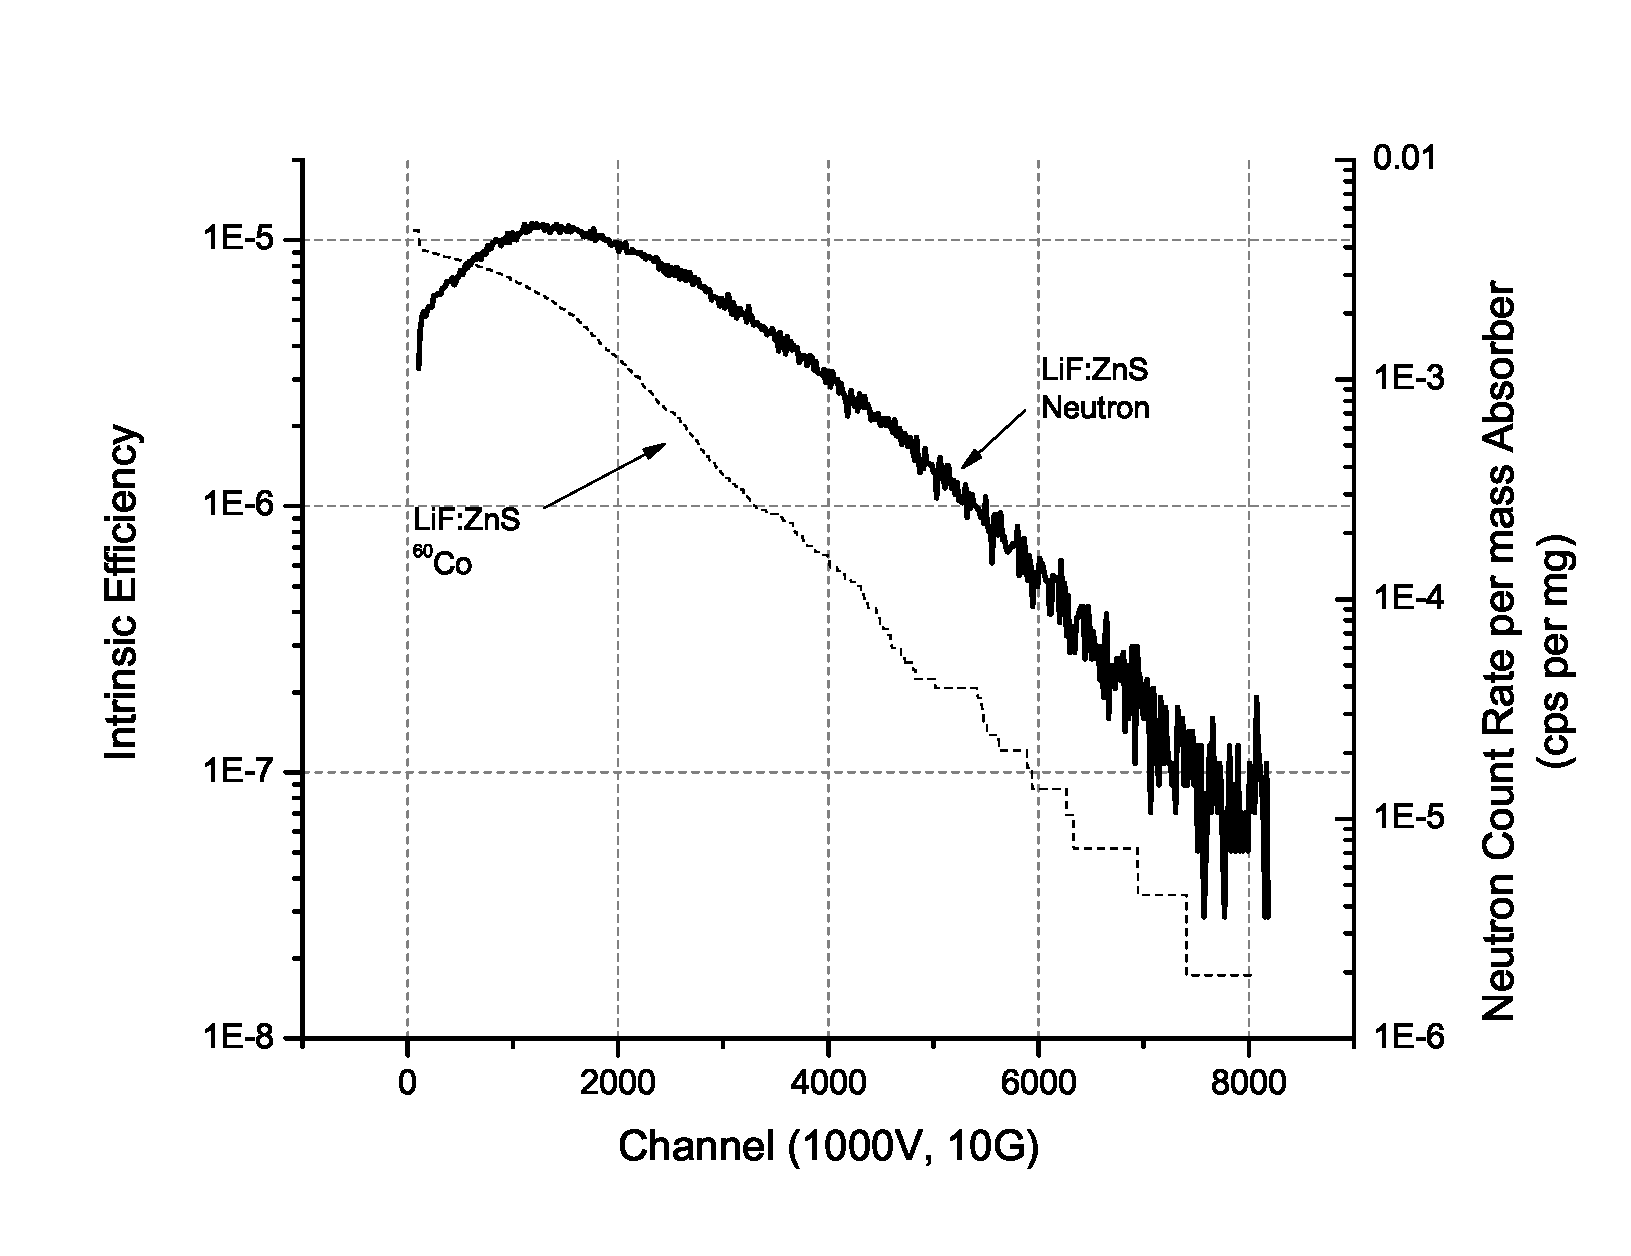
\includegraphics[width=\textwidth]{SC_EJ426_IntEff_CR}
  \caption[EJ 426 Performance]{Performance of EJ-426 HD2 (LiF:ZnS(Ag)) sheet.  This is the brightest scintillator tested, with the lowest gamma sensitivity.}
  \label{fig:EJ254Perf}
\end{figure}
\begin{figure}
  \centering
  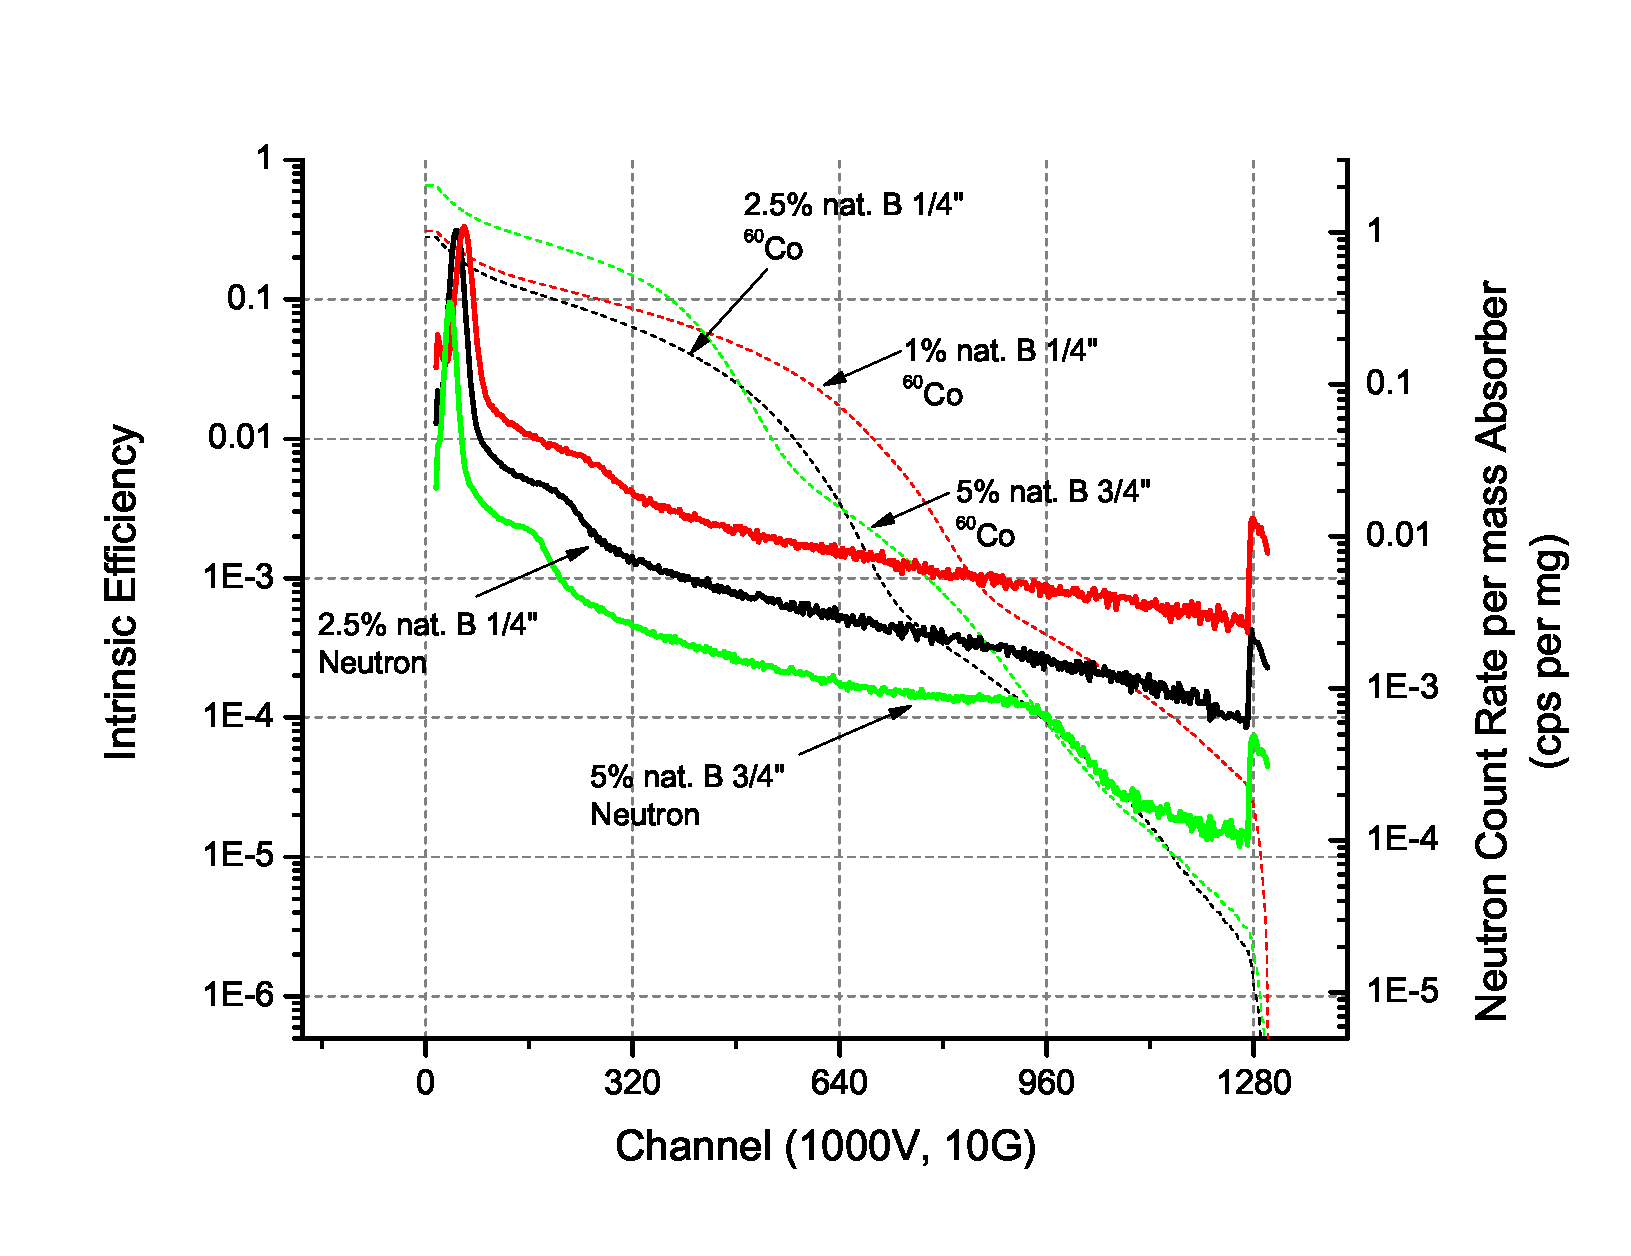
\includegraphics[width=\textwidth]{SC_EJ254_IntEff_CR}
  \caption[EJ 254 Performance]{Performance of EJ-254}
  \label{fig:EJ254Preformance}
\end{figure}
It is apparent that the EJ-254 is not a suitable candidate for replacement detector material in an RPM using a pulse height discriminator.
The reasons for this are twofold: 1) the detector is very thick which increases the probability of a gamma interaction as well as the probability that the interaction will deposit a majority of its energy and 2) \iso[10]{B} has a much lower Q-value (\SI{2.78}{\MeV} compared to \SI{4.78}{\MeV}) and a large pulse height deficit.
However, the material is optically transparent and due to \iso[10]{B}'s large thermal perhaps a thin sheet of EJ-254 might make a suitable detector material.
\subsection{Agreement to Previous Results}
It is observed from \autoref{fig:GuerardIntEff} (and supported by experience of the polystyrene films of different thickness) that the GS20 neutron spectra have the same endpoints while the gamma sensitivity increases with thickness.
If one assumes that the gamma sensitivity increases linearly with thickness (i.e. the first term in a exponential expansion), and then extrapolates it appears a \SI{2}{\mm} would then be expected to have a discrimination threshold for \num{1E-6} at 350 channels, at which point the neutron detection efficiency is less than a few percent.
This agrees with previous measurements of the fraction of counts above the MLLD for GS20, which tend to be about 4\%.

\section{Conclusions}
The post processed PEN and EJ-426 (LiF:ZnS(Ag)) detectors appear to be feasible detector materials for RPMs.
However, thin films of lithiated glass or boron loaded plastic may also be feasible replacement materials.
\section{Appendix}
The EJ-254, EJ-426, GS20, and post processed composite PEN spectra data contained in this report may be found at \verb+Dropbox/SpectraFiles/(0)_2013_Data/SampleComparison_28Apr2013+.
These files were measured from April 28, 2013 to May 2, 2013, with the voltage, gains and count times recorded in the lab notebook.
The 12 April 2013 PEN film as measured was replaced in this analysis with a PEN film of the sample compostion fabricated on 22 March 2013 as the 22 March 2013 had a higher total count rate, but a correspondingly lower count rate above the necessary discirmination threshold due to it's additional thickness.
In addition, the polystryene film was measured on the 12 April, 2013 and was then scaled by the ratio of the GS20 peak feature to 1,000V and 10G.
Of the spectra recorded, it was decided to go with Trial 1 when duplicate trials were made.
Corresponding hand calculations can be found on pages 104-106 of Matthew Urffer's 2nd lab book.
The script for scaling the spectra can be found in the following MATLAB code, where the data file is in the same location as the spectra.
This document is may be found in \LaTeX format at \url{\svnkw{HeadURL}}.  
The latest revision for this file is \svnrev, and was on \svndate, committed by \svnauthor.
\end{document}
